\chapter{Evaluation on other Techniques}

Transfer learning is only one way to improve performance with only a small amount of data. In this chapter, other techniques are explored that could prove valuable for the asbestos dataset like altering the size of the training data. Less but better quality images could lead to better performance, but also increasing the training data by adding the images from the validation set to the training set could provide a boost in performance. Cropping and resizing images can increase the dataset many fold. And last but not least, alterations to the networks will be done, in order to make the network smaller and thus more efficient or make the network able to cope with bigger input images.

\section{Evaluation Of Overall Number Of Parameters in VGG13}

In this section, I want to understand how the overall number of parameters affects the performance of the network. VGG13 was built primarily for the ImageNet Challenge and is probably too big for a task like the asbestos detection. In a first step, I will try to reduce the fully connected layers since they contribute to the complexity of the model the most. I will gradually reduce the number of parameters in the last 3 layers and compare the performance by averaging over 3 runs. Table \ref{tbl:vgg13_fc} shows the results. The last fully connected layer can safely be reduced from initially having 4096 units per layer to 16 units without harming the performance, or even increase it slightly while reducing the overall parameters by 92.39\%. It can be observed that applying transfer learning on a slightly altered architecture quickly diminishes it's advantages as expected. This can be explained because the architecture was relying on a specific configuration. Changing filters or fully connected layers might lead to having to retrain the whole architecture although the drop in performance is surprising since the changes only affect the last fully connected layers of the network and leave all previous filters intact.


\begin{table}[!h] \centering
\ra{1.3}
\caption{Variations in the last 3 fully connected layers of the VGG13 architecture. They were all performed with Batch Normalization. The last columne shows how much parameters remain in the varied architecture relative to the original VGG13 implementation.}
\resizebox{0.9\textwidth}{!}{%
\begin{tabular}{@{}rcccc@{}}
\toprule & Accuracy in \% (from scratch) & Accuracy in \% (pre-trained) & Number of Parameters & \% of Original \\
\midrule
VGG13\_4096    	& 81.06 $\pm$ 0.54 		& 88.04 $\pm$ 0.72 		& 128'959'042 	& 100\% \\
VGG13\_1024    	& 80.07 $\pm$ 0.72 		& 81.06 $\pm$ 0.72 		& 36'153'666 	& 28.04\% \\
VGG13\_512    		& 80.84 $\pm$ 0.78 		& 80.07 $\pm$ 0.27 		& 22'520'130 	& 17.46\% \\
VGG13\_256    		& 80.95 $\pm$ 0.87 		& 80.18 $\pm$ 0.87 		& 15'899'970 	& 12.33\% \\
VGG13\_128    		& 81.40 $\pm$ 0.98 		& 79.73 $\pm$ 1.41 		& 12'639'042 	& 9.80\% \\
VGG13\_64    		& 81.62 $\pm$ 0.41 		&  81.17 $\pm$ 0.41 		& 11'020'866 	& 8.55\% \\
VGG13\_32    		& 80.07 $\pm$ 2.36 		& 81.50 $\pm$ 0.56 		& 10'214'850 	& 7.92\% \\
\textbf{VGG13\_16}    & \textbf{82.06 $\pm$ 1.65} & \textbf{79.07 $\pm$ 0.81} & \textbf{9'812'610} & \textbf{7.61\%}\\
VGG13\_8    			& 78.74 $\pm$ 1.51 		& 80.18 $\pm$ 1.28 		& 9'611'682 		& 7.45\% \\
VGG13\_4    			& 79.73 $\pm$ 0.98 		& 80.18 $\pm$ 1.92 		& 9'511'266 		& 7.38\% \\
VGG13\_2    			& 59.80 $\pm$ 0.00 	& 74.31 $\pm$ 10.28 	& 9'461'070 		& 7.36\% \\
\bottomrule
\end{tabular}}
\label{tbl:vgg13_fc}
\end{table}

As a next step, the fully connected layer is held fixed at the original size of 4096 and the filters of all previous layers are reduced gradually. First, they are all halved until the first layer reaches 16 filters instead of the original 64. Then the layers deeper within the network are halved until all layers have 16 filters. After that configuration is reached, all filters all reduced gradually until only 2 filters per layer remain. Table \ref{tbl:vgg_filter_scheme} shows a summary of the filter reduction scheme. The last filter scheme "I" is to see if there is any benefit in increasing filters starting from 2 to the last layer. This imitates the original ratio of the filters but reducing the overall parameters drastically. \\


\begin{table}[!h] \centering
\ra{1.3}
\caption{Filter reduction scheme used on the original VGG13 architecture. The fully connected layer at the end is hold fixed and only the intermediate layers are reduced in filter size. The M stands for a max pooling layer.}
\resizebox{0.73\textwidth}{!}{%
\begin{tabular}{@{}rr@{}}
\toprule & VGG13 architecture variations in number of filters\\
\midrule
Original        & [64, 64, M, 128, 128, M, 256, 256, M, 512, 512, M, 512, 512, M]  \\
A                & [32, 32, M, 64, 64, M, 128, 128, M, 256, 256, M, 256, 256, M]  \\
B                & [16, 16, M, 32, 32, M, 64, 64, M, 128, 128, M, 128, 128, M]  \\
C                & [16, 16 M, 16, 16, M, 32, 32, M, 64, 64, M, 64, 64, M]  \\
D                & [16, 16, M, 16, 16, M, 16, 16, M, 32, 32, M, 32, 32, M]  \\
E                & [16, 16, M, 16, 16, M, 16, 16, M, 16, 16, M, 16, 16, M]  \\
F                & [8, 8, M, 8, 8, M, 8, 8, M, 8, 8, M, 8, 8, M]  \\
G                & [4, 4 M, 4, 4, M, 4, 4, M, 4, 4, M, 4, 4, M]  \\
H                & [2, 2, M, 2, 2, M, 2, 2, M, 2, 2, M, 2, 2, M]  \\
I                & [2, 2, M, 4, 4, M, 8, 8, M, 16, 16, M, 32, 32, M]  \\
J                & [2, 2, M, 4, 4, M, 8, 8, M, 16, 16, M, 32, 32, M]  \\
\bottomrule
\end{tabular}}
\label{tbl:vgg_filter_scheme}
\end{table}

The goal is to understand how the filters can be reduced and if a pattern can be observed. The results are summarized in Table \ref{tbl:vgg13_fc}. I can be shown that reducing the filters from the original schema to the scheme "A" does no harm the accuracy but reduces the trainable parameters by roughly 50\%. The standard deviation of 0.2721 gives a rather robust result and is lower than the standard deviation of 0.5425 obtained with the original scheme. Surprising is the result obtained with scheme "G" which uses only 4 filters per each layer reducing the overall parameters by 86.35\%. Although it's worse compared to the original scheme, it suffered only 1.7\% which could be attributed to chance. \\

\begin{table}[!h] \centering
\ra{1.3}
\caption{Variations in number of Filters throughout the VGG13 architecture as explained in table \ref{tbl:vgg_filter_scheme}.}
\resizebox{0.9\textwidth}{!}{%
\begin{tabular}{@{}rrrrr@{}}
\toprule & Accuracy in \% (from scratch) & Accuracy in \% (pre-trained) & Number of Parameters & \% of Original \\
\midrule
VGG13\_original 	& 81.06 $\pm$ 0.54 	& 88.04 $\pm$ 0.72 	& 128'959'042 	& 100\% \\
VGG13\_a    			& 81.06 $\pm$ 0.27	& 74.64 $\pm$ 4.46 & 70'529'186 	& 54.69\% \\
VGG13\_b    			& 80.40 $\pm$ 0.27 	& 80.18 $\pm$ 1.85 	& 43'073'874 	& 33.40\% \\
VGG13\_c    			& 78.74 $\pm$ 0.98	& 80.07 $\pm$ 0.98 & 29'790'002 	& 23.10\% \\
\textbf{VGG13\_d}    			& \textbf{79.40 $\pm$ 0.81} 	& \textbf{80.40 $\pm$ 0.47} & \textbf{23'261'010} 	& \textbf{18.04\%} \\
VGG13\_e    			& 78.96 $\pm$ 1.02 	& 79.73 $\pm$ 1.90	& 20'026'514 	& 15.53\% \\
VGG13\_f    			& 78.74 $\pm$ 0.81 	& 79.96 $\pm$ 0.68 	& 18'404'874 	& 14.27\% \\
\textbf{VGG13\_g}    			& \textbf{79.29 $\pm$ 0.68} 	& \textbf{79.29 $\pm$ 1.22} 	& \textbf{17'597'942} 	& \textbf{13.65\%} \\
VGG13\_h    			& 78.18 $\pm$ 0.41	& 78.63 $\pm$ 0.56 	& 17'195'448 	& 13.33\% \\
\midrule
VGG13\_i    			& 79.18 $\pm$ 2.21 	& 79.73 $\pm$ 1.18 	& 23'234'952 	& 18.02\% \\
\bottomrule
\end{tabular}}
\label{tbl:vgg13_fc}
\end{table}

Combining both modifications leads to yet another surprise as seen in Table \ref{tbl:vgg13_f_fc}. The modification with only 16 units per fully-connected layer and scheme "D" results in 80.73\% accuracy while reducing the overall complexity of the model by 99.946\%! The time needed to train the model drops from initially 1 hour and 13 minutes to only 25 minutes. Due to the heavy parallelization of the GPU's the drop in the time taken to learn is not linear at all. But more importantly is that the size of the model is much more deployable for production, e.g. IOT devices. \\


\begin{table}[!h] \centering
\ra{1.3}
\caption{Variations in number of Filters throughout the VGG13 architecture as explained in table \ref{tbl:vgg_filter_scheme}.}
\resizebox{0.9\textwidth}{!}{%
\begin{tabular}{@{}rcccc@{}}
\toprule & Accuracy in \% (from scratch) & Run time (hh:mm:ss) & Number of Parameters & \% of Original \\
\midrule
VGG13\_original    				& 81.06 $\pm$ 0.54 & 1:13:04 		& 128'959'042 	& 100\% \\
VGG13\_16\_a            			& 80.62 $\pm$ 1.25 & 0:27:01 		& 2'556'386 		& 1.9823\% \\
VGG13\_16\_b            			& 80.62 $\pm$ 0.63 & 0:25:37 		& 690'834 		& 0.5357\% \\
\textbf{VGG13\_16\_d}       	& \textbf{80.73 $\pm$ 1.44} & \textbf{0:25:35} & \textbf{70'290} & \textbf{0.0545\%} \\
\textbf{VGG13\_16\_g}       	& \textbf{79.29 $\pm$ 1.81} & \textbf{0:25:34} & \textbf{4'982} & \textbf{0.0039\%} \\
\midrule
\bottomrule
\end{tabular}}
\label{tbl:vgg13_f_fc}
\end{table}

Re-optimizing the hyperparameters with SigOpt yielded small improvements as seen in Table \ref{tbl:vgg13_f_fc_optimized}. \\


\begin{table}[!h] \centering
\ra{1.3}
\caption{SigOpt opimization VGG13 architecture as explained in table \ref{tbl:vgg_filter_scheme}.}
\resizebox{0.9\textwidth}{!}{%
\begin{tabular}{@{}rrrrr@{}}
\toprule & Accuracy (from scratch) & run time (hh:mm:ss) & Number of Parameters & \% of Original \\
\midrule
VGG13\_original    & 81.0631\% $\pm$ 0.5425 & 1:13:04 & 128'959'042 & 100\% \\
VGG13\_16\_d            & 81.2846\% $\pm$ 1.0963 & 0:25:34 & 70'290 & 0.0545\% \\
VGG13\_16\_g             & 80.0664\% $\pm$ 0.4698& 0:25:08 & 4'982 & 0.0039\% \\
\midrule
\bottomrule
\end{tabular}}
\label{tbl:vgg13_f_fc_optimized}
\end{table}

\subsection{Visualization of VGG}

First, let's visualize the architecture with the best results obtained which is the pre-trained vgg13 model with batch normalization. The Grad-CAM was taken on the last convolutional layer and can be seen in Figure \ref{fig:asbestos_gradcam}. 

\begin{figure}[!h]
\centering
\caption{Grad-CAM visualization applied on the left image once focusing on the areas that lead to the classification "non-asbestos" in the first row. And once focusing on the classification "asbestos" on the second row.}
\subfigure{
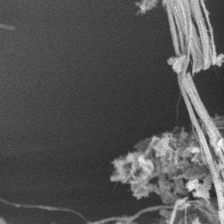
\includegraphics[width=.3\textwidth]{images/chapter6/vgg13/asbestos-original.png}
}
\subfigure{
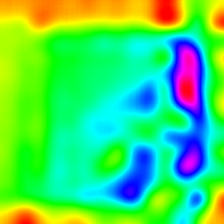
\includegraphics[width=.3\textwidth]{images/chapter6/vgg13/0-tl31-Cam-Heatmap.png}
}
\subfigure{
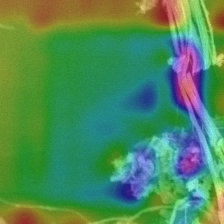
\includegraphics[width=.3\textwidth]{images/chapter6/vgg13/0-tl31-Cam-On-Image.png}
}

\subfigure{
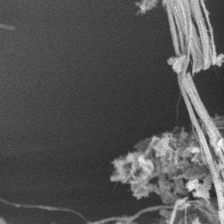
\includegraphics[width=.3\textwidth]{images/chapter6/vgg13/asbestos-original.png}
}
\subfigure{
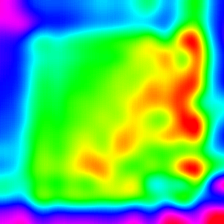
\includegraphics[width=.3\textwidth]{images/chapter6/vgg13/1-tl31-Cam-Heatmap.png}
}
\subfigure{
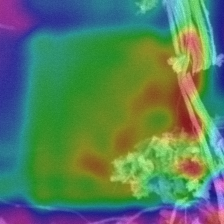
\includegraphics[width=.3\textwidth]{images/chapter6/vgg13/1-tl31-Cam-On-Image.png}
}
\label{fig:asbestos_gradcam}
\end{figure}

Although the asbestos is not clearly highlighted in the Grad-CAM visualization the two rows seen in Figure \ref{fig:asbestos_gradcam} show how the network looks for different patterns when classification for either category is done. As mentioned in the conclusion in chapter 5 the network probably uses feature maps that somehow resemble asbestos fibers and uses them to classify the images, thus leading to rather unclear feature maps. Also, it is possible that taking the last layer is detrimental for the asbestos task since the asbestos structure is not something as abstract and complex as a dog's face, thus the asbestos task could rely more on the low-level features. 

Visualizing images that activate certain filters in the last layer maximally are seen in Figure \ref{fig:vgg13_filter_activation}. The images are very similar to the visualizations on ImageNet with structures that do not resemble asbestos at all. Nonetheless, they achieve the best performance so far as explained in the previous chapter. I argue that some filter from ImageNet do indeed capture another structure in real life that resembles that of asbestos fibers, and if these very few filters are activated strongly. The classification is done on these very few filters and the rest (the big majority) is ignored. That's why reducing the last fully-connected layer to 16 units does not harm the performance at all.

\begin{figure}[!h]
\centering
\caption{Last Layer visualizations (8 of 512) of the pre-trained VGG13 with batch normalization.}
\subfigure{
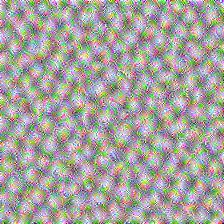
\includegraphics[width=.23\textwidth]{images/chapter6/vgg13/layers-pretrained/l22-f1.jpg}
}
\subfigure{
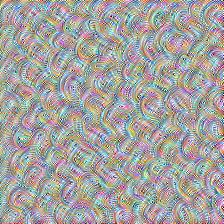
\includegraphics[width=.23\textwidth]{images/chapter6/vgg13/layers-pretrained/l22-f2.jpg}
}
\subfigure{
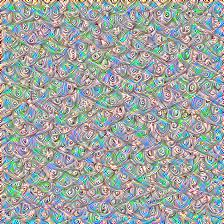
\includegraphics[width=.23\textwidth]{images/chapter6/vgg13/layers-pretrained/l22-f3.jpg}
}
\subfigure{
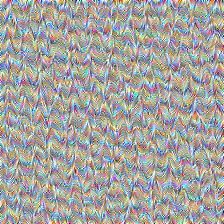
\includegraphics[width=.23\textwidth]{images/chapter6/vgg13/layers-pretrained/l22-f4.jpg}
}
\subfigure{
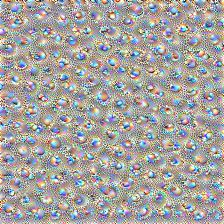
\includegraphics[width=.23\textwidth]{images/chapter6/vgg13/layers-pretrained/l22-f5.jpg}
}
\subfigure{
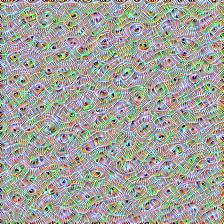
\includegraphics[width=.23\textwidth]{images/chapter6/vgg13/layers-pretrained/l22-f6.jpg}
}
\subfigure{
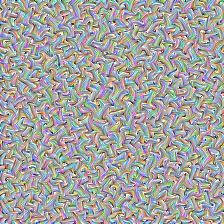
\includegraphics[width=.23\textwidth]{images/chapter6/vgg13/layers-pretrained/l22-f7.jpg}
}
\subfigure{
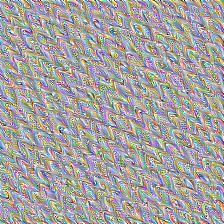
\includegraphics[width=.23\textwidth]{images/chapter6/vgg13/layers-pretrained/l22-f8.jpg}
}
\label{fig:vgg13_filter_activation}
\end{figure}

In order to contrast the original and pre-trained VGG13 with the modification performed on the VGG13 architecture with scheme "G" and only 16 units in the fully connected layers, I performed the same visualizations again. In Figure \ref{fig:asbestos_gradcam_g} Grad-CAM visualizations with heatmaps over the image are shown for the last convolution layer. As before the first row shows what areas responsible for the classification "non-asbestos", and the second row shows what areas are responsible for the classification "asbestos".

\begin{figure}[!h]
\centering
\caption{GradCam visualization applied on the left image once with looking for asbestos structures (right) and once looking for not-asbestos structures (middle).}
\subfigure{
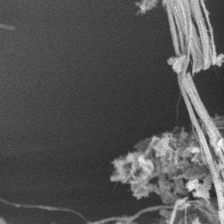
\includegraphics[width=.3\textwidth]{images/chapter6/vgg13/asbestos-original.png}
}
\subfigure{
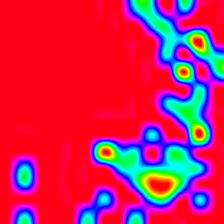
\includegraphics[width=.3\textwidth]{images/chapter6/vgg13/layers-g-16/0-tl31-Cam-Heatmap.png}
}
\subfigure{
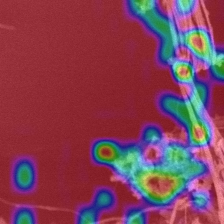
\includegraphics[width=.3\textwidth]{images/chapter6/vgg13/layers-g-16/0-tl31-Cam-On-Image.png}
}
\subfigure{
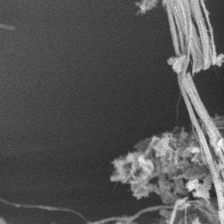
\includegraphics[width=.3\textwidth]{images/chapter6/vgg13/asbestos-original.png}
}
\subfigure{
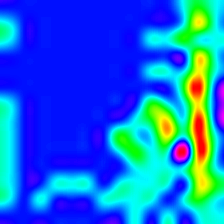
\includegraphics[width=.3\textwidth]{images/chapter6/vgg13/layers-g-16/1-tl31-Cam-Heatmap.png}
}
\subfigure{
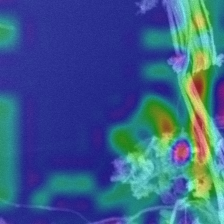
\includegraphics[width=.3\textwidth]{images/chapter6/vgg13/layers-g-16/1-tl31-Cam-On-Image.png}
}
\label{fig:asbestos_gradcam_g}
\end{figure}

The visualizations from Figure \ref{fig:asbestos_gradcam} need to be taken very critically. I suspect that modifying the architecture to that extent might have had an unexpected impact on the visualization library. Some visualizations of lower convolution layers don't succeed at all and yield unusable results.

As shown with the original model, Figure \ref{fig:vgg13_g_filter_activation} lists 4 layer visualizations performed from the last convolution layer from the modified VGG13 architecture. As already seen in chapter five, contrary to the pre-trained mode, no complex patterns can be found and that holds true for every filter throughout the model. In the appendix, all 40 filters of the architecture are shown for comparison.

\begin{figure}[!h]
\centering
\caption{Last Layer visualizations (4 of 4) of the VGG13\_16\_g architecture trained from scratch and with batch normalization.}
\subfigure{

\includegraphics[width=.23\textwidth]{images/chapter6/vgg13/layers-fs/l31-f0.jpg}
}
\subfigure{

\includegraphics[width=.23\textwidth]{images/chapter6/vgg13/layers-fs/l31-f1.jpg}
}
\subfigure{

\includegraphics[width=.23\textwidth]{images/chapter6/vgg13/layers-fs/l31-f2.jpg}
}
\subfigure{

\includegraphics[width=.23\textwidth]{images/chapter6/vgg13/layers-fs/l31-f3.jpg}
}
\label{fig:vgg13_g_filter_activation}
\end{figure}











\section{Evaluation Of Overall Number Of Parameters in ResNet18}

Although VGG13 is the biggest network regarding the number of learnable parameters (over 128 million), ResNet18 in its original form also has quite many parameters (over 11 million). It has also been built to recognize 1'000 classes from ImageNet, which even distinguishes different breeds of dogs, and therefore is probably too big and too complex for the asbestos task. That is not to say, that the task is simple in its nature, but that asbestos has a common looking structure and the networks hard work is to find this structure in many different settings and under difficult conditions. Reducing the number of filters has another huge benefit of reducing the overall number of trainable parameters and thus speeding up the learning process, using less memory and being much easier to deploy on productive configurations.\\

For the above-mentioned reason, the ResNet18 implementation has been altered to contain only a certain amount of filters in every single layer. The amount has been set to different values ranging from 1 to 32 filters. With 32 filters of size 3x3, only 320 parameters are used per layer. In ResNet18, for example, there are 4 blocks of 2 layers of 320 parameters making in total 2560 parameters. That does not yet count in the first 7x7 convolution and the fully-connected layer with its softmax function but the number of parameters is reduced dramatically as shown in Table \ref{tbl:resnet18-different-filters}. The original version increases its layers from the initial 3 channels of an image to 64, 128, 256 and 512 filters up to the fully connected layer. The fully connected layer thus again makes a big bulk of all trainable parameters. Keeping the filters constant does reduce the number of trainable parameters within the network and automatically also reduces the parameters in the last fully connected layer.

Since observations on VGG13 have shown that pre-training is not helpful in this scenario, it has been omitted with ResNet18.


\begin{table}[!h] \centering
\ra{1.3}
\caption{Resnet18 with different number of filters on the FINAL dataset. The number of filters present in paranthesis is the number of filters used per layer.}
\resizebox{0.79\textwidth}{!}{%
\begin{tabular}{@{}rrrrr@{}}
\toprule & accuracy (from scratch) & trainable parameters &  param reduction (\%) \\
\midrule
ResNet18 (official)            & 79.62\% &  11'177'538 & 100\%     \\
ResNet18 (32 filters)            & 78.405\% &  156'578 & 1.4008\%    \\
ResNet18 (16 filters)            & 81.06\% &  40'658 & 0.3637\%    \\
ResNet18 (8 filters)            & 79.402\% &  10'922 & 0.0977\%     \\
ResNet18 (4 filters)            & 79.62\% &  3'110 & 0.0278\%     \\
ResNet18 (2 filters)            & 80.066\% &  968 & 0.0087\%    \\
ResNet18 (1 filter)                & 75.083\% &  338 & 0.0030\%     \\
\bottomrule
\end{tabular}}
\label{tbl:resnet18-different-filters}
\end{table}

It is very surprising that reducing the learnable parameters by 99.64\% for the ResNet18 modification with 16 filters yields better results for the asbestos task trained from scratch. It does indeed confirm the hypothesis that for binary classification of a mineral the current models are way too big and wasteful. Also, the ResNet18 modification with only 2 filters per layer (reduction of parameters by 99.99\%) outperforms the original ResNet18 architecture.






\section{Evaluation Of Different Dataset Sizes And Variations}

All the different dataset variations are compared against each other within the same architecture. Each result is obtained by running the model three times and averaging over all runs. DeepDIVA has a script that randomly distributes the images into one of the three sets. It is important to note, that once the sets have been created, the test set has never been altered. It stays the same for all dataset variations. Table \ref{tbl:resnet18_dataset} shows the results for ResNet18. \\

\begin{table}[!h] \centering
\ra{1.3}
\caption{Dataset variations with ResNet18. The first column shows how the datasets performed when trained from scratch whereas the second column shows how the datasets performed with pre-training.}
\resizebox{0.79\textwidth}{!}{%
\begin{tabular}{@{}rccc@{}}
\toprule & accuracy in \% (from scratch) & accuracy in \% (pre-trained) &   $\Delta$ \\
\midrule
FINAL                        	& 79.62  $\pm$ 0.95 	& 86.93 $\pm$ 0.78 		& +7.31  \\
FINAL\_C                   	& 80.73 $\pm$ 0.38 		& 84.05 $\pm$ 0.96 	& +3.32 \\
FINAL\_C\_B            	& 81.39 $\pm$ 1.38 		& 85.27 $\pm$ 0.80 		& +3.88 \\
FINAL\_CH                	& 81.62 $\pm$ 0.29 		& 84.94 $\pm$ 0.40 	& +3.32 \\
FINAL\_CH\_B           	& 80.73 $\pm$ 0.84 		& 85.05 $\pm$ 0.33 		& +4.32 \\
FINAL\_EXTENDED   	& 81.06 $\pm$ 0.38 		& 84.50 $\pm$ 0.86 	& +3.44 \\
\bottomrule
\end{tabular}}
\label{tbl:resnet18_dataset}
\end{table}

\quad

Changing the train set by reducing questionable and unclear images has lead to consistent improvements in the ResNet18 model trained from scratch but to consistently worse results when training from pre-trained weights. A possible explanation could be that training from scratch needs a higher quality of the data sets meaning no wrongly labeled images and no images with obvious errors in them. That would not explain why the model with transfer learning performs consistently worse with different training and validation sets. In Table \ref{tbl:densenet121_dataset} the summary shows how DenseNet121 reacts with different datasets. \\


\begin{table}[!h] \centering
\ra{1.3}
\caption{Dataset variations with DenseNet121. The first column shows how the datasets performed when trained from scratch whereas the second column shows how the datasets performed with pre-training.}
\resizebox{0.79\textwidth}{!}{%
\begin{tabular}{@{}rccc@{}}
\toprule & accuracy in \% (from scratch) & accuracy in \% (pre-trained) &   $\Delta$ \\
\midrule
FINAL                    		& 83.72 $\pm$ 1.20 		& 86.16 $\pm$ 1.17   	& +2.44     \\
FINAL\_C             		& 82.61 $\pm$ 0.97 		& 83.94 $\pm$ 0.59 	& +1.33 \\
FINAL\_C\_B        		& 80.39 $\pm$ 0.38 	& 85.38 $\pm$ 0.19 		& +4.99 \\
FINAL\_CH				& 79.61 $\pm$ 2.23 		& 86.60 $\pm$ 0.40 	& +6.99 \\
FINAL\_CH\_B          	& 83.17 $\pm$ 0.11		& 84.37 $\pm$ 0.81 		& +1.20 \\
FINAL\_EXTENDED	& 83.06 $\pm$ 1.03 		& 85.60 $\pm$ 2.12 		& +2.54 \\
\bottomrule
\end{tabular}}
\label{tbl:densenet121_dataset}
\end{table}

With Densenet121 there is no improvement to be seen by changing the dataset. If trained from scratch all variations lead to slightly worse results. If trained with pre-trained weights, the FINAL\_CH dataset yields marginally better accuracy but that is most likely due to chance. In Table \ref{fig:inceptionv3_dataset} the summary shows how Inception v3 behaves with different datasets.

\begin{table}[!h] \centering
\ra{1.3}
\caption{Dataset variations with Inception v3. The first group shows how the datasets performed when trained from scratch whereas the second group shows how the datasets performed with pre-training. FINAL\_C\_B died for the non-pre-trained twice. Only one datapoint used.}
\resizebox{0.79\textwidth}{!}{%
\begin{tabular}{@{}rccc@{}}
\toprule & accuracy in \% (from scratch) & accuracy in \% (pre-trained) &   $\Delta$ \\
\midrule
FINAL                        & 82.83  $\pm$ 0.62 		& 85.93 $\pm$ 0.40  	& +3.10  \\
FINAL\_C                   & 80.4 $\pm$ 0.69 		& 85.82 $\pm$  0.29 	& +5.42 \\
FINAL\_C\_B              & 82.06 $\pm$ 1.77 		& 85.27 $\pm$  1.57 		& +3.21 \\
FINAL\_CH                 & 81.06 $\pm$ 0.54 		& 85.71 $\pm$ 0.27 		& +4.65 \\
FINAL\_CH\_B            & 81.06 $\pm$ 0.38 		& 85.27 $\pm$  1.22 		& +4.21 \\
FINAL\_EXTENDED   & 81.72 $\pm$ 0.38 		& 84.16 $\pm$ 0.44 		& +2.44 \\
\bottomrule
\end{tabular}}
\label{tbl:inceptionv3_dataset}
\end{table}

For the inception v3 architecture trained from scratch and trained with pre-trained weights, there is a very slight but constant disadvantage to using different datasets which I cannot make sense of. Removing images with errors or adding the validation images to the training set should increase overall accuracy, but this increase is never significantly observed.












\section{Evaluation Of Different Cropping And Augmentation Methods}

In chapter 5, strong overfitting was observed in the training set. ResNet18 with transfer learning, for example, converged in only about 5 epochs to nearly 100\% accuracy on the training set and stayed there as seen in Figure \ref{fig:resnet18-graph}. The accuracy from the test set showed that this accuracy was due to overfitting. In order to mitigate this problem, several cropping and resizing methods will be used on ResNet18 with the goal of reducing overfitting on training and increasing generalization and thus achieving better results on the test set. Also, some randomness through random flipping and mirroring is introduced. As for the dataset, only the FINAL variation is used for this part.

\subsection{Randomness}

Here, random cropping is performed first in order to crop the image to the smallest image height in the dataset which is 768 pixels this already allows vertical and horizontal randomness leading to every epoch training on different augmented images. Then the image is resized to the expected input size of the network being 224x224 pixels for ResNet18. With resizing a  smaller image then the original image, less information is lost due to the resizing process, which is a good thing. In the end, two transformations happen with a probability of 0.5: flipping horizontally and flipping vertically. All transformations are performed on the training set only. One run was performed as usual with 50 epochs and a  learning rate decay every 20 epochs. Since data augmentation yields new images to train from every epoch, there is much more variation and less overfitting. Therefore another 3 runs have been performed with 100 epochs and a learning rate decay every  30 epochs. The summary of these is shown in Table \ref{tbl:ResNet18_cropping}: \\


\begin{table}[!h] \centering
\ra{1.3}
\caption{Cropping, resizing and  random flipping performed on the ResNet18 architecture with and without transfer learning. The first row is a run with the original configuration without any randomness or cropping and serves as comparison.}
\resizebox{0.79\textwidth}{!}{%
\begin{tabular}{@{}rrrr@{}}
\toprule & Accuracy in \% (from scratch) & Accuracy in \% (pre-trained) &   $\Delta$ in \% \\
\midrule
ResNet18 original & 79.62  $\pm$ 0.95 &  85.83 $\pm$ 0.41 & +6.21     \\
\midrule
ResNet18 (50 epochs) & 81.73  $\pm$ 1.09 &  84.83 $\pm$ 0.78 & +3.10     \\
ResNet18 (100 epochs) &  81.17 $\pm$ 0.87 & 85.93 $\pm$ 0.32 & +4.76 \\
\bottomrule
\end{tabular}}
\label{tbl:ResNet18_cropping}
\end{table}

Unfortunately, the improvement in accuracy of only 2.11\% for the ResNet18 trained from scratch with simple data augmentation is not as high as expected. From the model with the pre-trained weights, it even gets worse with a decrease of exactly 1\%. But as seen in Graph \ref{fig:resnet18-da-graph} no overfitting takes place for the model trained from scratch and less overfitting is found in the pre-trained model. This is in strong contrast to Figure \ref{fig:resnet18-graph} from Chapter 5.

\begin{figure}[!h]
\centering
\caption{Training and validation graphs for ResNet18 with simple data augmentation. Once with pre-trained weights from ImageNet and once trained from scratch.}
\subfigure{
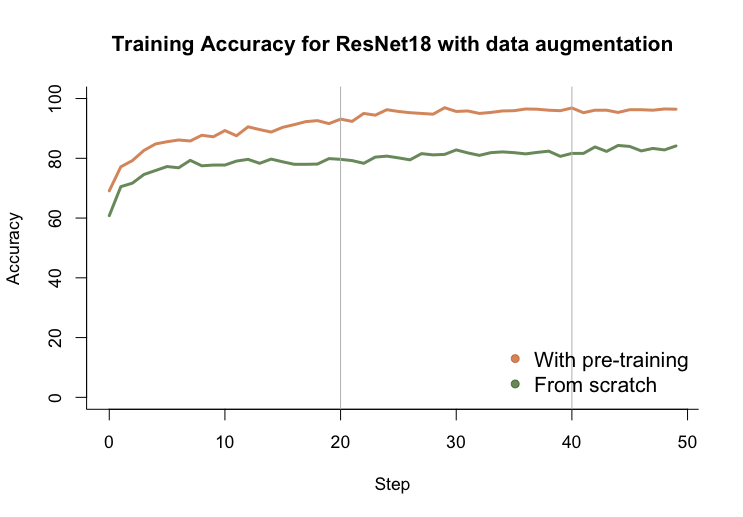
\includegraphics[width=.46\textwidth]{images/chapter6/resnet18-da/TA-resnet18-da.png}
}
\subfigure{
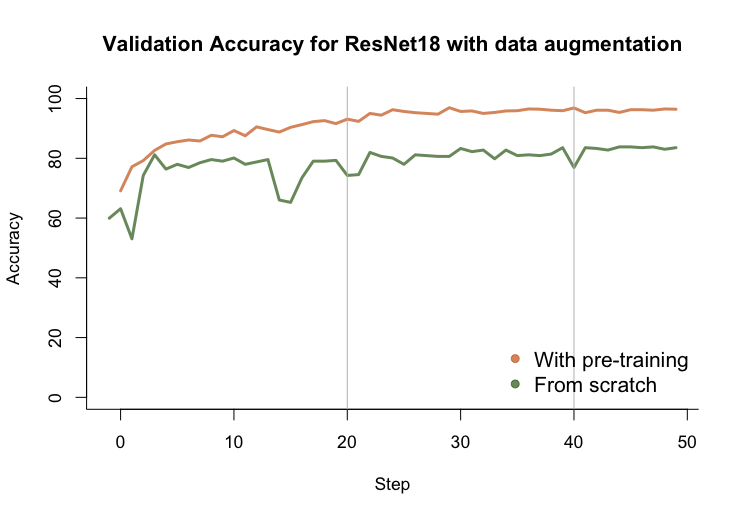
\includegraphics[width=.46\textwidth]{images/chapter6/resnet18-da/VA-resnet18-da.png}
}
\label{fig:resnet18-da-graph}
\end{figure}

Convergence happens at roughly the same amount of epochs. The model trained from scratch does never catch up with the pre-trained model which has already been attributed to the more complex feature mappings of the pre-trained model. A very interesting point can be seen in Table \ref{tbl:ResNet18_cropping_different_acc} where on the first two rows the ResNet runs are shown as performed in Chapter 5. Severe overfitting happens for the pre-trained model after only a few epochs and after the model trained from scratch towards the end. But both are near 100\% accuracy for the training. The validation accuracy is much more realistic since it does only test the network on this data. Validation and test set accuracies should be near each other. For the ResNet18 architecture with cropping and 50 epochs no overfitting can be observed. The training accuracy remains around 82\% for training, validation and test sets. This simple data augmentation is enough to create new images for roughly 50 epochs, but not for 100 epochs. Although there is some randomness introduced, it is not sophisticated enough.

\begin{table}[!h] \centering
\ra{1.3}
\caption{Different set accuracies. If the training accuracy is much higher than the validation or test accuracy, then there is a problem with overfitting to the training data.}
\resizebox{0.85\textwidth}{!}{%
\begin{tabular}{@{}rccc@{}}
\toprule & Accuracy train set in \% & Accuracy validation set in \% &  Accuracy test set in \% \\
\midrule
ResNet18 original (from scratch)			& 99.28   		&  77.83 	& 79.62     \\
ResNet18 original (pre-trained)				& 100.00   	&  88.61 	& 85.83     \\
\midrule
ResNet18 (50 epochs / from scratch)	& 83.33   		&  82.25 	& 81.73   \\
ResNet18 (50 epochs / pre-trained)		& 95.85   		&  88.57 	& 84.83     \\
\midrule
ResNet18 (100 epochs / from scratch)	& 84.70   		&  83.22 	& 81.17     \\
ResNet18 (100 epochs / pre-trained)	 	&  98.07 		& 87.57 	& 85.93 \\
\bottomrule
\end{tabular}}
\label{tbl:ResNet18_cropping_different_acc}
\end{table}

\subsection{FiveCrop}

The torch library comes with a FiveCrop implementation which could be used with minor changes in the code. The FiveCrop implementation crops 5 images of a given size from the whole image. All corners and the center are cropped. In training and evaluation, these crops are stacked on top of each other and fed to the network. The output is averaged across all crops before the weights get updated. Table \ref{resnet18-fivecrop} summarizes the results.\\


\begin{table}[!h] \centering
\ra{1.3}
\caption{Resnet18 FiveCrop Implementation with and without pre-training. FINAL (regular) means ResNet18 with the resizing of the image instead of cropping and averaging}
\resizebox{0.79\textwidth}{!}{%
\begin{tabular}{@{}rccc@{}}
\toprule & Accuracy in \% (from scratch) & Accuracy in \% (pre-trained) &   $\Delta$ in \%  \\
\midrule
FINAL (regular)          	& 79.62  $\pm$ 0.95 	& 86.93 $\pm$ 0.78   	& +7.31     \\
FINAL (fiveCrop)          	& 82.28 $\pm$ 1.81 		& 87.93 $\pm$ 1.49 		& +5.65   \\
\midrule
Accuracy gain				& +2.66						& +1.00 						& - \\
\bottomrule
\end{tabular}}
\label{tbl:resnet18-fivecrop}
\end{table}

With FiveCrop slightly better results are achieved than without data augmentation. The increase for the model trained from scratch is 2.66\% whereas the increase for the pre-trained model is 1\%. No overfitting is taking place. The training, validation and test accuracies are all around 83\% for the model trained from scratch. For the pre-trained model, the training accuracy is around 91\% which is slightly overfitting. Validation and test accuracies are both around 88\%.

\subsection{NineCrop}

The NineCrop is an own implementation that puts more weight on the center of the image. The nine crops taken from the image are all symmetrically positioned around the center with only minimal or none overlap. Taking nine crops instead of five is not without disadvantages. If many crops end up having no asbestos in them it will rather harm than improve the learning process. Table \ref{tbl:resnet18-randomnine} summarizes the results.

\begin{table}[!h] \centering
\ra{1.3}
\caption{Resnet18 FiveCrop Implementation with and without pre-training. FINAL (regular) means ResNet18 with the resizing of the image instead of cropping and averaging}
\resizebox{0.79\textwidth}{!}{%
\begin{tabular}{@{}rccc@{}}
\toprule & Accuracy in \% (from scratch) & Accuracy in \% (pre-trained) &   $\Delta$ in \% \\
\midrule
FINAL (regular)              		& 79.62  $\pm$ 0.95 	& 86.93 $\pm$ 0.78		& +7.31    \\
FINAL (randomNine)          & 83.39 $\pm$ 0.95 		& 87.92 $\pm$ 1.13 		& +4.53    \\
\midrule
Accuracy gain					& +3.77							& +1.00 						& - \\
\bottomrule
\end{tabular}}
\label{tbl:resnet18-randomnine}
\end{table}



\section{Evaluation of Different Image Size Inputs to the network}

The input size of the network ranges relative to the architectures from 224x224 pixels for ResNet to 299x299 pixels for inception v3. Resizing the image inevitably leads to a loss of information. Therefore one path of investigation was to check if it is possible to change the architecture in a certain way, that allows for bigger images to be fed into the network. Images are highly compressed in jpg or png format but when they are loaded into tensors or arrays they increase their size drastically which leads to the problem of not having enough memory. Therefore, the ResNet18 architecture with 16 filters throughout the network has been used, to allow for bigger images. No transfer learning could be applied for that reason. In order to accommodate bigger input images into the network, convolutional layers have been added on top of the network that halves the input volume and prepares the image for the previous first layer of 224x224 pixels. For the ResNet18\_448 modification the added code is shown in the following listing:

\begin{minipage}{\linewidth}
\begin{lstlisting}[language=Python, caption=Python example, basicstyle=\tiny]
        self.expected_input_size = (448, 448)

        # ************************************************************************************************
        self.conv00 = nn.Conv2d(3, constant_number_of_filters, kernel_size=7, stride=2, padding=3,
                                bias=False)
        self.bn00 = nn.BatchNorm2d(constant_number_of_filters)
        # ************************************************************************************************
\end{lstlisting}
\end{minipage}

The forward pass consists of doing first the new convolution with batch normalization, then passing the output through a ReLU and then feeding it to the previously first convolution layer that expects the original size. Table \ref{tbl:resnet18-different-input} summarizes the results.

\begin{table}[!h] \centering
\ra{1.3}
\caption{Different image input sizes are fed into ResNet18 architectuers with only 16 filters per layer. The first layers of the network have been adapted to allow bigger input images}
\resizebox{0.79\textwidth}{!}{%
\begin{tabular}{@{}rrr@{}}
\toprule & accuracy (from scratch) & accuracy (pre-trained) \\
\midrule
FINAL (regular 224)                & 79.62\%  $\pm$ 0.9465 &   86.93\% $\pm$ 0.7757     \\
FINAL (input 448)            & 77.41\% $\pm$ 1.6940   & -     \\
FINAL (input 896)            & 79.62\% $\pm$ 0.6827   & -     \\
FINAL (input 1024)            & 80.62\% $\pm$ 0.8287   & -     \\
\bottomrule
\end{tabular}}
\label{tbl:resnet18-different-input}
\end{table}

Increasing the input size from 224x224 pixels to 448x448 pixels decreased the overall accuracy by roughly 2\%. Increasing it to 896x896 achieved the exact same accuracy with a lower standard deviation and increasing it to the full size of the image increased the accuracy by almost 1\%. Overall I expected better results but all the networks have been carefully crafted by their creators and simply adding convolutions on top of it does alter the network in quite unpredictable ways. For the ResNet18\_1024 modification I had to add 8 convolution layers and 8 batch normalization in order to get the input volume down to 224x224x16 (with 16 filters) which looks like this:

\begin{minipage}{\linewidth}
\begin{lstlisting}[language=Python, caption=Python example, basicstyle=\tiny]
self.expected_input_size = (1024, 1024)

        # ************************************************************************************************
        self.conv01 = nn.Conv2d(3, constant_number_of_filters, kernel_size=7, stride=2,
                                padding=3, bias=False)
        self.bn01 = nn.BatchNorm2d(constant_number_of_filters)

        self.conv02 = nn.Conv2d(constant_number_of_filters, constant_number_of_filters, kernel_size=7, stride=2,
                                padding=3, bias=False)
        self.bn02 = nn.BatchNorm2d(constant_number_of_filters)

        # 256
        self.conv03 = nn.Conv2d(constant_number_of_filters, constant_number_of_filters, kernel_size=7, stride=1,
                                padding=0, bias=False)
        self.bn03 = nn.BatchNorm2d(constant_number_of_filters)

        # 250

        self.conv04 = nn.Conv2d(constant_number_of_filters, constant_number_of_filters, kernel_size=7, stride=1,
                                padding=0, bias=False)
        self.bn04 = nn.BatchNorm2d(constant_number_of_filters)

        # 244

        self.conv05 = nn.Conv2d(constant_number_of_filters, constant_number_of_filters, kernel_size=7, stride=1,
                                padding=0, bias=False)
        self.bn05 = nn.BatchNorm2d(constant_number_of_filters)

        # 238

        self.conv06 = nn.Conv2d(constant_number_of_filters, constant_number_of_filters, kernel_size=7, stride=1,
                                padding=0, bias=False)
        self.bn06 = nn.BatchNorm2d(constant_number_of_filters)

        # 232

        self.conv07 = nn.Conv2d(constant_number_of_filters, constant_number_of_filters, kernel_size=7, stride=1,
                                padding=0, bias=False)
        self.bn07 = nn.BatchNorm2d(constant_number_of_filters)

        # 226

        self.conv08 = nn.Conv2d(constant_number_of_filters, constant_number_of_filters, kernel_size=3, stride=1,
                                padding=0, bias=False)
        self.bn08 = nn.BatchNorm2d(constant_number_of_filters)

        # 224

        # ************************************************************************************************
\end{lstlisting}
\end{minipage}

This makes it so much harder to train this network since there are 9 convolution layers before the actual ResNet18 architecture starts. There are no skip connections in the first 9 layers and therefore the vanishing/exploding gradient problem starts to play a role again.


\section{Conclusion}

Several modifications have been performed on VGG13 and ResNet18 architectures in order to squeeze out more accuracy on the test set. VGG13's last layer got reduced to 16 units creating a much smaller architecture of only 7.61\% of its original size, increasing accuracy to 82.06\%. Then going through different filter schema it was observed, that further reduction of the parameters is still possible with only a minor decrease in accuracy. Overall it may be said that the original architectures were built for discriminating between 1'000 classes some of which were very similar to each other. For the asbestos recognition task that is clearly unnecessary.

Reducing the overall number of parameters makes transfer learning not applicable anymore since most of the useful filters are lost due to the reduction. The same behavior was observed with ResNet18 where a reduction by 99.99\% of the learnable parameters still leads to the same accuracy. Further decrease leads to worse accuracies.

Variations in the dataset didn't yield the expected boost in performance. It was hoped that removing clear errors from the dataset would make the training process easier but that was not the case. What surprised, even more, was that the extension of the data set by adding the validation images to the training images didn't improve the overall performance. This could be due to the images not being correctly classified and the data set quality that does not allow for better performance since the 90\% mark was never broken on a regular basis regardless of all the changes.

Data augmentation was able to reduce overfitting in a regular 50 epoch run and lead to marginally better performance. Training, validation and test sets all reached roughly the same accuracy which was the goal of this task. The boost in performance through better generalization was not achieved as hoped for.

Modifying the architecture in order to allow for bigger image input did lead to a marginal improvement only for the last modification where the full image was fed into the network. Unfortunately, the filters had to be reduced to only 16 for such big images to process making transfer learning unavailable.

